\documentclass[twoside]{book}

% Packages required by doxygen
\usepackage{fixltx2e}
\usepackage{calc}
\usepackage{doxygen}
\usepackage[export]{adjustbox} % also loads graphicx
\usepackage{graphicx}
\usepackage[utf8]{inputenc}
\usepackage{makeidx}
\usepackage{multicol}
\usepackage{multirow}
\PassOptionsToPackage{warn}{textcomp}
\usepackage{textcomp}
\usepackage[nointegrals]{wasysym}
\usepackage[table]{xcolor}

% Font selection
\usepackage[T1]{fontenc}
\usepackage[scaled=.90]{helvet}
\usepackage{courier}
\usepackage{amssymb}
\usepackage{sectsty}
\renewcommand{\familydefault}{\sfdefault}
\allsectionsfont{%
  \fontseries{bc}\selectfont%
  \color{darkgray}%
}
\renewcommand{\DoxyLabelFont}{%
  \fontseries{bc}\selectfont%
  \color{darkgray}%
}
\newcommand{\+}{\discretionary{\mbox{\scriptsize$\hookleftarrow$}}{}{}}

% Page & text layout
\usepackage{geometry}
\geometry{%
  a4paper,%
  top=2.5cm,%
  bottom=2.5cm,%
  left=2.5cm,%
  right=2.5cm%
}
\tolerance=750
\hfuzz=15pt
\hbadness=750
\setlength{\emergencystretch}{15pt}
\setlength{\parindent}{0cm}
\setlength{\parskip}{3ex plus 2ex minus 2ex}
\makeatletter
\renewcommand{\paragraph}{%
  \@startsection{paragraph}{4}{0ex}{-1.0ex}{1.0ex}{%
    \normalfont\normalsize\bfseries\SS@parafont%
  }%
}
\renewcommand{\subparagraph}{%
  \@startsection{subparagraph}{5}{0ex}{-1.0ex}{1.0ex}{%
    \normalfont\normalsize\bfseries\SS@subparafont%
  }%
}
\makeatother

% Headers & footers
\usepackage{fancyhdr}
\pagestyle{fancyplain}
\fancyhead[LE]{\fancyplain{}{\bfseries\thepage}}
\fancyhead[CE]{\fancyplain{}{}}
\fancyhead[RE]{\fancyplain{}{\bfseries\leftmark}}
\fancyhead[LO]{\fancyplain{}{\bfseries\rightmark}}
\fancyhead[CO]{\fancyplain{}{}}
\fancyhead[RO]{\fancyplain{}{\bfseries\thepage}}
\fancyfoot[LE]{\fancyplain{}{}}
\fancyfoot[CE]{\fancyplain{}{}}
\fancyfoot[RE]{\fancyplain{}{\bfseries\scriptsize Generated by Doxygen }}
\fancyfoot[LO]{\fancyplain{}{\bfseries\scriptsize Generated by Doxygen }}
\fancyfoot[CO]{\fancyplain{}{}}
\fancyfoot[RO]{\fancyplain{}{}}
\renewcommand{\footrulewidth}{0.4pt}
\renewcommand{\chaptermark}[1]{%
  \markboth{#1}{}%
}
\renewcommand{\sectionmark}[1]{%
  \markright{\thesection\ #1}%
}

% Indices & bibliography
\usepackage{natbib}
\usepackage[titles]{tocloft}
\setcounter{tocdepth}{3}
\setcounter{secnumdepth}{5}
\makeindex

% Hyperlinks (required, but should be loaded last)
\usepackage{ifpdf}
\ifpdf
  \usepackage[pdftex,pagebackref=true]{hyperref}
\else
  \usepackage[ps2pdf,pagebackref=true]{hyperref}
\fi
\hypersetup{%
  colorlinks=true,%
  linkcolor=blue,%
  citecolor=blue,%
  unicode%
}

% Custom commands
\newcommand{\clearemptydoublepage}{%
  \newpage{\pagestyle{empty}\cleardoublepage}%
}

\usepackage{caption}
\captionsetup{labelsep=space,justification=centering,font={bf},singlelinecheck=off,skip=4pt,position=top}

%===== C O N T E N T S =====

\begin{document}

% Titlepage & ToC
\hypersetup{pageanchor=false,
             bookmarksnumbered=true,
             pdfencoding=unicode
            }
\pagenumbering{alph}
\begin{titlepage}
\vspace*{7cm}
\begin{center}%
{\Large Login.\+py }\\
\vspace*{1cm}
{\large Generated by Doxygen 1.8.14}\\
\end{center}
\end{titlepage}
\clearemptydoublepage
\pagenumbering{roman}
\tableofcontents
\clearemptydoublepage
\pagenumbering{arabic}
\hypersetup{pageanchor=true}

%--- Begin generated contents ---
\chapter{Hierarchical Index}
\section{Class Hierarchy}
This inheritance list is sorted roughly, but not completely, alphabetically\+:\begin{DoxyCompactList}
\item Q\+Dialog\begin{DoxyCompactList}
\item \contentsline{section}{Login.\+Login\+Window}{\pageref{classLogin_1_1LoginWindow}}{}
\end{DoxyCompactList}
\end{DoxyCompactList}

\chapter{Class Index}
\section{Class List}
Here are the classes, structs, unions and interfaces with brief descriptions\+:\begin{DoxyCompactList}
\item\contentsline{section}{\hyperlink{classNetworking_1_1Networking__Hardware}{Networking.\+Networking\+\_\+\+Hardware} }{\pageref{classNetworking_1_1Networking__Hardware}}{}
\item\contentsline{section}{\hyperlink{classNetworking_1_1Networking__Python}{Networking.\+Networking\+\_\+\+Python} }{\pageref{classNetworking_1_1Networking__Python}}{}
\end{DoxyCompactList}

\chapter{Class Documentation}
\hypertarget{classLogin_1_1LoginWindow}{}\section{Login.\+Login\+Window Class Reference}
\label{classLogin_1_1LoginWindow}\index{Login.\+Login\+Window@{Login.\+Login\+Window}}
Inheritance diagram for Login.\+Login\+Window\+:\begin{figure}[H]
\begin{center}
\leavevmode
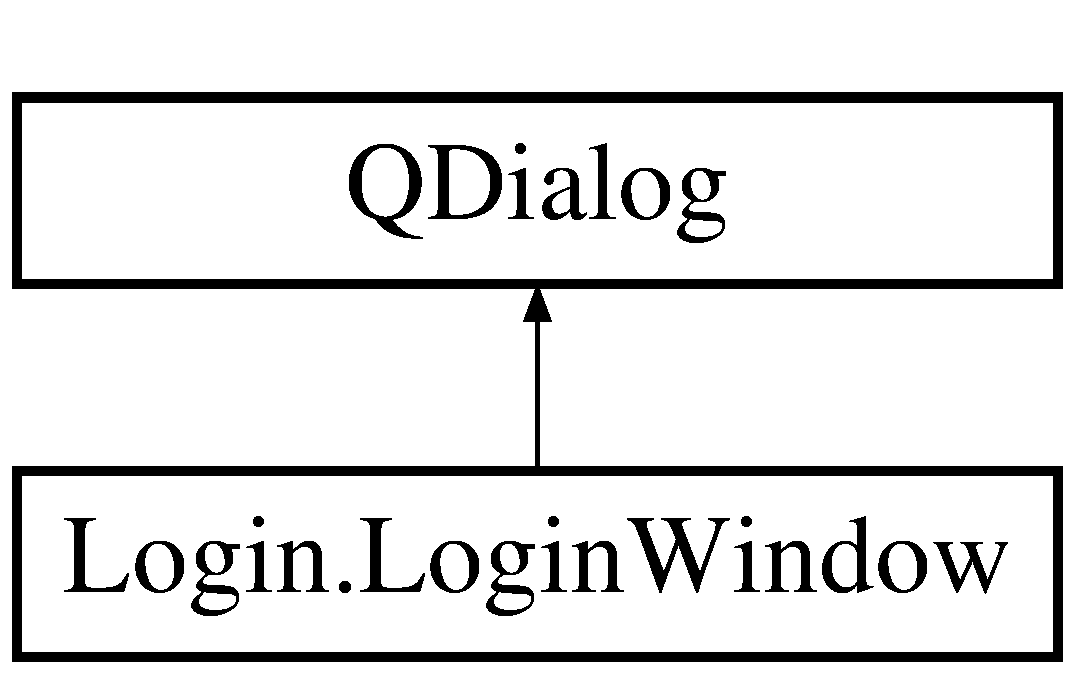
\includegraphics[height=2.000000cm]{classLogin_1_1LoginWindow}
\end{center}
\end{figure}
\subsection*{Public Member Functions}
\begin{DoxyCompactItemize}
\item 
def \hyperlink{classLogin_1_1LoginWindow_aef57c8863324399070faf514e2883e66}{\+\_\+\+\_\+init\+\_\+\+\_\+} (self, parent=None)
\item 
def \hyperlink{classLogin_1_1LoginWindow_a391e97589387c5760c2d62f29b8ff1d3}{handle\+Login} (self)
\end{DoxyCompactItemize}
\subsection*{Public Attributes}
\begin{DoxyCompactItemize}
\item 
\mbox{\Hypertarget{classLogin_1_1LoginWindow_af399a91c1b7b6375a1b01def88da385e}\label{classLogin_1_1LoginWindow_af399a91c1b7b6375a1b01def88da385e}} 
{\bfseries login\+\_\+filter}
\item 
\mbox{\Hypertarget{classLogin_1_1LoginWindow_aa87869ad002d2120d438e91df3a954e0}\label{classLogin_1_1LoginWindow_aa87869ad002d2120d438e91df3a954e0}} 
{\bfseries password\+\_\+filter}
\item 
\mbox{\Hypertarget{classLogin_1_1LoginWindow_a53dacafcf67eda9debcab4e1377c99a9}\label{classLogin_1_1LoginWindow_a53dacafcf67eda9debcab4e1377c99a9}} 
{\bfseries login\+\_\+label}
\item 
\mbox{\Hypertarget{classLogin_1_1LoginWindow_aff1354ca874c366e8ca8ba4c9af1574f}\label{classLogin_1_1LoginWindow_aff1354ca874c366e8ca8ba4c9af1574f}} 
{\bfseries text\+Name}
\item 
\mbox{\Hypertarget{classLogin_1_1LoginWindow_afa642ee1b28a5eab79994873513a3a2f}\label{classLogin_1_1LoginWindow_afa642ee1b28a5eab79994873513a3a2f}} 
{\bfseries text\+Pass}
\item 
\mbox{\Hypertarget{classLogin_1_1LoginWindow_a496b8df8778cf173a80583fb29f6cb83}\label{classLogin_1_1LoginWindow_a496b8df8778cf173a80583fb29f6cb83}} 
{\bfseries button\+Login}
\item 
\mbox{\Hypertarget{classLogin_1_1LoginWindow_a9db82f6715afbc939356324d5b0a3d24}\label{classLogin_1_1LoginWindow_a9db82f6715afbc939356324d5b0a3d24}} 
{\bfseries data}
\end{DoxyCompactItemize}
\subsection*{Static Public Attributes}
\begin{DoxyCompactItemize}
\item 
string {\bfseries style}
\end{DoxyCompactItemize}


\subsection{Detailed Description}
\begin{DoxyVerb}This class handles the login window. This is the window that appears
when the user first opens the application. This is needed because all the data
the program processes should be uploaded to the user's account.
\end{DoxyVerb}
 

\subsection{Constructor \& Destructor Documentation}
\mbox{\Hypertarget{classLogin_1_1LoginWindow_aef57c8863324399070faf514e2883e66}\label{classLogin_1_1LoginWindow_aef57c8863324399070faf514e2883e66}} 
\index{Login\+::\+Login\+Window@{Login\+::\+Login\+Window}!\+\_\+\+\_\+init\+\_\+\+\_\+@{\+\_\+\+\_\+init\+\_\+\+\_\+}}
\index{\+\_\+\+\_\+init\+\_\+\+\_\+@{\+\_\+\+\_\+init\+\_\+\+\_\+}!Login\+::\+Login\+Window@{Login\+::\+Login\+Window}}
\subsubsection{\texorpdfstring{\+\_\+\+\_\+init\+\_\+\+\_\+()}{\_\_init\_\_()}}
{\footnotesize\ttfamily def Login.\+Login\+Window.\+\_\+\+\_\+init\+\_\+\+\_\+ (\begin{DoxyParamCaption}\item[{}]{self,  }\item[{}]{parent = {\ttfamily None} }\end{DoxyParamCaption})}

\begin{DoxyVerb}This is an intializer used to  intialize the fields that are required for the login screen
In particular it initializes:

       1.Login filter
       2.Password Filter
       3.Username Area
       4.Password Area
       5.Login Button\end{DoxyVerb}
 

\subsection{Member Function Documentation}
\mbox{\Hypertarget{classLogin_1_1LoginWindow_a391e97589387c5760c2d62f29b8ff1d3}\label{classLogin_1_1LoginWindow_a391e97589387c5760c2d62f29b8ff1d3}} 
\index{Login\+::\+Login\+Window@{Login\+::\+Login\+Window}!handle\+Login@{handle\+Login}}
\index{handle\+Login@{handle\+Login}!Login\+::\+Login\+Window@{Login\+::\+Login\+Window}}
\subsubsection{\texorpdfstring{handle\+Login()}{handleLogin()}}
{\footnotesize\ttfamily def Login.\+Login\+Window.\+handle\+Login (\begin{DoxyParamCaption}\item[{}]{self }\end{DoxyParamCaption})}

\begin{DoxyVerb}Handles Login submission by posting to server.
Confirms the user has entered a username
It attempts to login to the server.
If user ID is found, user is logged in.
Otherwise displays warning message.\end{DoxyVerb}
 

\subsection{Member Data Documentation}
\mbox{\Hypertarget{classLogin_1_1LoginWindow_a1893950a27b708cf283b86f9a55d107a}\label{classLogin_1_1LoginWindow_a1893950a27b708cf283b86f9a55d107a}} 
\index{Login\+::\+Login\+Window@{Login\+::\+Login\+Window}!style@{style}}
\index{style@{style}!Login\+::\+Login\+Window@{Login\+::\+Login\+Window}}
\subsubsection{\texorpdfstring{style}{style}}
{\footnotesize\ttfamily string Login.\+Login\+Window.\+style\hspace{0.3cm}{\ttfamily [static]}}

{\bfseries Initial value\+:}
\begin{DoxyCode}
= \textcolor{stringliteral}{'''}
\textcolor{stringliteral}{QLabel}
\textcolor{stringliteral}{\{}
\textcolor{stringliteral}{    font-family: Times New Roman;}
\textcolor{stringliteral}{    font-size: 18pt;}
\textcolor{stringliteral}{\}}
\textcolor{stringliteral}{'''}
\end{DoxyCode}


The documentation for this class was generated from the following file\+:\begin{DoxyCompactItemize}
\item 
Login.\+py\end{DoxyCompactItemize}

%--- End generated contents ---

% Index
\backmatter
\newpage
\phantomsection
\clearemptydoublepage
\addcontentsline{toc}{chapter}{Index}
\printindex

\end{document}
